\documentclass[UTF8]{ctexart}
\usepackage[a4paper,margin=1.8cm]{geometry}
\usepackage{graphicx}
\usepackage{float}
\usepackage{longtable}
\usepackage{array}
\usepackage{xcolor}
\usepackage{fancyvrb}
\usepackage{hyperref}
\setlength{\parindent}{0pt}
\setlength{\parskip}{0.45em}
\begin{document}
\section*{剩余知识点题型适配模拟卷}

\subsection*{卷面说明}

本卷只针对前面四套卷没有完全展开的 PPT 内容。题型按知识点适合方式安排。本版采用“题目后紧跟按考试标准重写答案”的排版，便于复习时对照。

\begin{Verbatim}[fontsize=\small,breaklines=true]
1. 背景型知识点：适合简答、判断、对比。
2. 理论细节：适合解释原因、说明规则。
3. 过程型知识点：适合小计算、小推导。
4. 次级但可出题内容：适合短流程题。
\end{Verbatim}

\subsection*{一、背景型简答：IR、NFA/DFA、SSA（20 分）}

\subsubsection*{题目}

回答下列问题：

1. 说明高层 IR 和低层 IR 的区别，各举一个特点。 2. 说明为什么 DFA 的执行通常比 NFA 的直接模拟更简单。 3. 说明 SSA 为什么有利于优化。 4. 说明工业编译器中使用 SSA 或类似 SSA 形式的原因。

\subsubsection*{按考试标准重写答案}

\paragraph*{1. 高层 IR 和低层 IR 的区别}

答题时要从“离源程序近还是离机器近”来区分：

\begin{longtable}{|p{0.23\linewidth}|p{0.23\linewidth}|p{0.23\linewidth}|p{0.23\linewidth}|}
\hline
类型 & 特点 & 适合阶段 & 例子 \\
\hline
\endfirsthead
类型 & 特点 & 适合阶段 & 例子 \\
\hline
\endhead
高层 IR & 保留较多源语言结构，如循环、函数、对象、异常等 & 前端语义分析、高层优化 & AST、带结构化控制流的 IR \\
\hline
低层 IR & 更接近目标机器，显式表示跳转、load/store、寄存器、栈等 & 后端代码生成、寄存器分配、指令选择 & 接近汇编的三地址码或机器 IR \\
\hline
\end{longtable}

因此，高层 IR 的优点是语义信息丰富；低层 IR 的优点是便于映射到机器指令。

\paragraph*{2. DFA 为什么比 NFA 直接模拟更简单}

核心差异是“当前状态数量”：

\begin{longtable}{|p{0.47\linewidth}|p{0.47\linewidth}|}
\hline
自动机 & 读入一个字符时的状态变化 \\
\hline
\endfirsthead
自动机 & 读入一个字符时的状态变化 \\
\hline
\endhead
DFA & 从一个当前状态唯一转移到下一个状态 \\
\hline
NFA & 可能从一组当前状态转移到另一组状态，还要处理 epsilon 转移 \\
\hline
\end{longtable}

DFA 执行伪代码只需要：

\begin{Verbatim}[fontsize=\small,breaklines=true]
state = start
for ch in input:
  state = delta(state, ch)
\end{Verbatim}

NFA 直接模拟时需要维护状态集合：

\begin{Verbatim}[fontsize=\small,breaklines=true]
states = epsilon-closure({start})
for ch in input:
  states = epsilon-closure(move(states, ch))
\end{Verbatim}

所以 DFA 的实现更直接，运行时只维护一个当前状态。

\paragraph*{3. SSA 为什么有利于优化}

SSA 的规则是每个变量版本只赋值一次。这样定义点和使用点关系清楚：

\begin{longtable}{|p{0.47\linewidth}|p{0.47\linewidth}|}
\hline
优化 & SSA 带来的便利 \\
\hline
\endfirsthead
优化 & SSA 带来的便利 \\
\hline
\endhead
常量传播 & 一个版本若定义为常量，可直接沿 def-use 链传播 \\
\hline
死代码删除 & 若某个定义版本没有使用点，可以删除 \\
\hline
公共子表达式消除 & 操作数版本明确，判断两个表达式是否相同更容易 \\
\hline
数据流分析 & 不必反复区分同名变量的不同定义 \\
\hline
\end{longtable}

例子：

\begin{Verbatim}[fontsize=\small,breaklines=true]
x1 = 1
x2 = x1 + 2
y1 = x2
\end{Verbatim}

\texttt{x1}、\texttt{x2} 是不同版本，优化器能明确 \texttt{x2} 依赖 \texttt{x1}，不会把不同赋值混在一起。

\paragraph*{4. 工业编译器使用 SSA 或类似形式的原因}

工业编译器要做大量优化，SSA 能把数据依赖显式化，降低实现复杂度。典型流程是：

\begin{Verbatim}[fontsize=\small,breaklines=true]
普通 IR -> 构造 SSA -> 在 SSA 上做优化 -> 消除 phi -> 进入后端
\end{Verbatim}

后端不能直接保留抽象 \texttt{phi} 函数，通常会把它展开为前驱边上的复制指令，再结合寄存器分配做合并。

\subsection*{二、理论细节：SDD、SDT、属性文法（20 分）}

\subsubsection*{题目}

回答下列问题：

1. 说明 SDD 和 SDT 的区别。 2. 说明属性文法和带副作用语义动作的区别。 3. 为什么属性依赖图中存在环时，属性值无法正常求值。 4. 什么是受控副作用，写出两个基本要求。

\subsubsection*{按考试标准重写答案}

\paragraph*{1. SDD 和 SDT 的区别}

\begin{longtable}{|p{0.23\linewidth}|p{0.23\linewidth}|p{0.23\linewidth}|p{0.23\linewidth}|}
\hline
概念 & 中文名 & 关注点 & 表达形式 \\
\hline
\endfirsthead
概念 & 中文名 & 关注点 & 表达形式 \\
\hline
\endhead
SDD & 语法制导定义 & “属性怎么算” & 给产生式配属性方程 \\
\hline
SDT & 语法制导翻译 & “动作何时执行” & 把语义动作嵌入产生式右部 \\
\hline
\end{longtable}

SDD 更像规格说明，SDT 更接近实现。可以先写 SDD，再根据分析顺序把属性计算和语义动作安排成 SDT。

\paragraph*{2. 属性文法和带副作用语义动作的区别}

\begin{longtable}{|p{0.31\linewidth}|p{0.31\linewidth}|p{0.31\linewidth}|}
\hline
对比项 & 属性文法 & 带副作用语义动作 \\
\hline
\endfirsthead
对比项 & 属性文法 & 带副作用语义动作 \\
\hline
\endhead
主要方式 & 通过属性方程计算值 & 执行动作并修改外部状态 \\
\hline
外部状态 & 通常不依赖修改全局结构 & 可能修改符号表、输出代码、更新计数器 \\
\hline
分析重点 & 属性依赖是否有合法求值顺序 & 动作执行时机是否正确、是否重复 \\
\hline
\end{longtable}

例子：

\begin{Verbatim}[fontsize=\small,breaklines=true]
T.type = int
\end{Verbatim}

是属性计算；

\begin{Verbatim}[fontsize=\small,breaklines=true]
addType(id.name, T.type)
\end{Verbatim}

会修改符号表，是带副作用动作。

\paragraph*{3. 依赖图中存在环时为什么无法正常求值}

属性依赖图的边表示“先算谁，再算谁”。若有环：

\begin{Verbatim}[fontsize=\small,breaklines=true]
A.x -> B.y -> A.x
\end{Verbatim}

则 \texttt{A.x} 要等 \texttt{B.y}，同时 \texttt{B.y} 又要等 \texttt{A.x}。此时不存在拓扑序，无法安排一个合法的属性求值先后顺序。

\begin{longtable}{|p{0.31\linewidth}|p{0.31\linewidth}|p{0.31\linewidth}|}
\hline
图结构 & 是否可拓扑排序 & 属性能否按顺序求值 \\
\hline
\endfirsthead
图结构 & 是否可拓扑排序 & 属性能否按顺序求值 \\
\hline
\endhead
无环 & 可以 & 可以 \\
\hline
有环 & 不可以 & 不能按普通属性方程求值 \\
\hline
\end{longtable}

\paragraph*{4. 受控副作用及基本要求}

受控副作用是指语义动作虽然修改外部结构，但修改发生在明确、可预测、满足依赖关系的位置。

基本要求：

\begin{longtable}{|p{0.47\linewidth}|p{0.47\linewidth}|}
\hline
要求 & 含义 \\
\hline
\endfirsthead
要求 & 含义 \\
\hline
\endhead
所需属性已计算 & 例如 \texttt{addType(id.name,T.type)} 必须等 \texttt{T.type} 已知 \\
\hline
执行位置固定 & 不能因分析策略不同而提前或延后到错误位置 \\
\hline
不引入依赖环 & 副作用不能让属性互相等待 \\
\hline
不重复、不漏执行 & 特别是声明插入、代码输出等动作 \\
\hline
错误可恢复 & 发生重复声明等错误时符号表仍保持一致 \\
\hline
\end{longtable}

\subsection*{三、过程型小题：LR 表格驱动分析器（20 分）}

\subsubsection*{题目}

已知某 LR 分析表有如下条目：

\begin{Verbatim}[fontsize=\small,breaklines=true]
ACTION[0,id] = s1
ACTION[1,+]  = r(E -> id)
ACTION[1,$]  = r(E -> id)
ACTION[2,+]  = s3
ACTION[2,$]  = acc
ACTION[3,id] = s4
ACTION[4,$]  = r(E -> E + id)

GOTO[0,E] = 2
\end{Verbatim}

输入串：

\begin{Verbatim}[fontsize=\small,breaklines=true]
id + id $
\end{Verbatim}

要求：

1. 说明 ACTION 表和 GOTO 表分别在什么时候使用。 2. 写出分析过程中栈和输入的大致变化。 3. 说明什么时候接受输入。

\subsubsection*{按考试标准重写答案}

\paragraph*{1. ACTION 表和 GOTO 表什么时候用}

LR 分析器每一步都看“状态栈顶状态”和“当前输入符号”：

\begin{longtable}{|p{0.23\linewidth}|p{0.23\linewidth}|p{0.23\linewidth}|p{0.23\linewidth}|}
\hline
表 & 下标 & 使用时机 & 表项含义 \\
\hline
\endfirsthead
表 & 下标 & 使用时机 & 表项含义 \\
\hline
\endhead
ACTION & \texttt{[状态, 终结符]} & 当前要处理输入符号时 & 移进、规约、接受或报错 \\
\hline
GOTO & \texttt{[状态, 非终结符]} & 规约出某个非终结符之后 & 决定压入的新状态 \\
\hline
\end{longtable}

动作解释：

\begin{Verbatim}[fontsize=\small,breaklines=true]
s1：移进当前输入符号，并压入状态 1。
r(E -> id)：把栈顶与产生式右部 id 对应的内容弹出，规约成 E。
acc：接受输入串。
\end{Verbatim}

\paragraph*{2. 分析过程}

输入串：

\begin{Verbatim}[fontsize=\small,breaklines=true]
id + id $
\end{Verbatim}

完整表格如下：

\begin{longtable}{|p{0.19\linewidth}|p{0.19\linewidth}|p{0.19\linewidth}|p{0.19\linewidth}|p{0.19\linewidth}|}
\hline
步骤 & 状态栈 & 符号栈 & 剩余输入 & 查表与动作 \\
\hline
\endfirsthead
步骤 & 状态栈 & 符号栈 & 剩余输入 & 查表与动作 \\
\hline
\endhead
1 & \texttt{0} & 空 & \texttt{id + id \textbackslash{}\$} & \texttt{ACTION[0,id]=s1}，移进 \texttt{id} \\
\hline
2 & \texttt{0 1} & \texttt{id} & \texttt{+ id \textbackslash{}\$} & \texttt{ACTION[1,+]=r(E -> id)}，规约 \\
\hline
3 & \texttt{0 2} & \texttt{E} & \texttt{+ id \textbackslash{}\$} & 规约后查 \texttt{GOTO[0,E]=2} \\
\hline
4 & \texttt{0 2} & \texttt{E} & \texttt{+ id \textbackslash{}\$} & \texttt{ACTION[2,+]=s3}，移进 \texttt{+} \\
\hline
5 & \texttt{0 2 3} & \texttt{E +} & \texttt{id \textbackslash{}\$} & \texttt{ACTION[3,id]=s4}，移进 \texttt{id} \\
\hline
6 & \texttt{0 2 3 4} & \texttt{E + id} & \texttt{\textbackslash{}\$} & \texttt{ACTION[4,\textbackslash{}\$]=r(E -> E + id)}，规约 \\
\hline
7 & \texttt{0 2} & \texttt{E} & \texttt{\textbackslash{}\$} & 规约后回到状态 0 查 \texttt{GOTO[0,E]=2} \\
\hline
8 & \texttt{0 2} & \texttt{E} & \texttt{\textbackslash{}\$} & \texttt{ACTION[2,\textbackslash{}\$]=acc}，接受 \\
\hline
\end{longtable}

第 6 步规约 \texttt{E -> E + id} 时，右部长度为 3，所以弹出符号栈中的 \texttt{E + id} 和对应的 3 个状态，再把 \texttt{E} 压入，并按弹出后的状态查 GOTO。

\paragraph*{3. 什么时候接受输入}

接受条件不是“输入刚好读完”本身，而是：

\begin{Verbatim}[fontsize=\small,breaklines=true]
当前状态 = 2
当前输入符号 = $
ACTION[2,$] = acc
\end{Verbatim}

因此当状态栈为 \texttt{0 2}、符号栈为 \texttt{E}、剩余输入为 \texttt{\textbackslash{}\$} 时，分析器接受输入串。

\subsection*{四、次级流程题：通用左递归消除（20 分）}

\subsubsection*{题目}

文法：

\begin{Verbatim}[fontsize=\small,breaklines=true]
S -> A a | b
A -> S d | c
\end{Verbatim}

按非终结符顺序：

\begin{Verbatim}[fontsize=\small,breaklines=true]
S, A
\end{Verbatim}

1. 判断该文法是否存在间接左递归。 2. 按通用左递归消除思路，先把 \texttt{A -> S d} 中的 \texttt{S} 用 \texttt{S} 的产生式替换。 3. 消除替换后 \texttt{A} 的直接左递归。

\subsubsection*{按考试标准重写答案}

\paragraph*{1. 判断间接左递归}

原文法：

\begin{Verbatim}[fontsize=\small,breaklines=true]
S -> A a | b
A -> S d | c
\end{Verbatim}

如果某个非终结符能经过一步或多步推导重新以自己开头，就是左递归。这里：

\begin{Verbatim}[fontsize=\small,breaklines=true]
S => A a
  => S d a
\end{Verbatim}

因此 \texttt{S} 存在间接左递归。\texttt{A} 也可以推出：

\begin{Verbatim}[fontsize=\small,breaklines=true]
A => S d
  => A a d
\end{Verbatim}

所以这个文法确实存在间接左递归。

\paragraph*{2. 按顺序 `S, A` 替换}

通用算法按非终结符顺序处理。处理 \texttt{S} 时，前面没有非终结符，不替换。

处理 \texttt{A} 时，产生式中有：

\begin{Verbatim}[fontsize=\small,breaklines=true]
A -> S d
\end{Verbatim}

因为 \texttt{S} 在顺序中排在 \texttt{A} 前面，所以要把 \texttt{S} 的右部代入：

\begin{Verbatim}[fontsize=\small,breaklines=true]
S -> A a | b
\end{Verbatim}

代入 \texttt{A -> S d} 得：

\begin{Verbatim}[fontsize=\small,breaklines=true]
A -> A a d | b d
\end{Verbatim}

再保留原来的 \texttt{A -> c}：

\begin{Verbatim}[fontsize=\small,breaklines=true]
A -> A a d | b d | c
\end{Verbatim}

\paragraph*{3. 消除 `A` 的直接左递归}

现在 \texttt{A} 的产生式分成两类：

\begin{longtable}{|p{0.31\linewidth}|p{0.31\linewidth}|p{0.31\linewidth}|}
\hline
类型 & 产生式 & 记号 \\
\hline
\endfirsthead
类型 & 产生式 & 记号 \\
\hline
\endhead
左递归部分 & \texttt{A -> A a d} & \texttt{alpha = a d} \\
\hline
非左递归部分 & \texttt{A -> b d}、\texttt{A -> c} & \texttt{beta1 = b d}，\texttt{beta2 = c} \\
\hline
\end{longtable}

套用规则：

\begin{Verbatim}[fontsize=\small,breaklines=true]
A  -> beta A'
A' -> alpha A' | epsilon
\end{Verbatim}

得到：

\begin{Verbatim}[fontsize=\small,breaklines=true]
A  -> b d A' | c A'
A' -> a d A' | epsilon
\end{Verbatim}

最终文法为：

\begin{Verbatim}[fontsize=\small,breaklines=true]
S  -> A a | b
A  -> b d A' | c A'
A' -> a d A' | epsilon
\end{Verbatim}

注意：\texttt{S -> A a | b} 保留不变，因为本题指定按顺序 \texttt{S, A} 处理，替换发生在处理 \texttt{A} 时。

\subsection*{五、次级流程题：数组类型的 L 属性定义（20 分）}

\subsubsection*{题目}

考虑数组类型声明：

\begin{Verbatim}[fontsize=\small,breaklines=true]
T -> B C
B -> int | float
C -> [ num ] C | epsilon
\end{Verbatim}

设计一个 L 属性 SDD，用于计算类型 \texttt{T.type}。要求：

1. \texttt{B.type} 表示基本类型。 2. \texttt{C.in} 表示从左侧传入的已有类型。 3. \texttt{C.type} 表示加上数组维度后的类型。 4. 对声明形式 \texttt{int[10][20]} 写出类型构造顺序。

\subsubsection*{按考试标准重写答案}

\paragraph*{1. 属性含义}

题目已经规定属性方向，按这个方向设计：

\begin{longtable}{|p{0.47\linewidth}|p{0.47\linewidth}|}
\hline
属性 & 含义 \\
\hline
\endfirsthead
属性 & 含义 \\
\hline
\endhead
\texttt{B.type} & 基本类型，如 \texttt{int}、\texttt{float} \\
\hline
\texttt{C.in} & 从左侧传入的当前已构造类型 \\
\hline
\texttt{C.type} & 处理完当前及后续数组维度后的类型 \\
\hline
\texttt{T.type} & 整个类型表达式的最终类型 \\
\hline
\end{longtable}

\paragraph*{2. L 属性 SDD}

\begin{Verbatim}[fontsize=\small,breaklines=true]
T -> B C
  C.in = B.type
  T.type = C.type

B -> int
  B.type = int

B -> float
  B.type = float

C -> [ num ] C1
  C1.in = array(num.val, C.in)
  C.type = C1.type

C -> epsilon
  C.type = C.in
\end{Verbatim}

该定义是 L 属性定义，因为 \texttt{C.in} 只依赖左侧兄弟 \texttt{B.type} 或父结点传下来的属性，不依赖右侧兄弟。

\paragraph*{3. `int[10][20]` 的类型构造顺序}

按题目给定的继承属性方向，从左到右构造：

\begin{longtable}{|p{0.31\linewidth}|p{0.31\linewidth}|p{0.31\linewidth}|}
\hline
步骤 & 产生式或动作 & 得到的类型 \\
\hline
\endfirsthead
步骤 & 产生式或动作 & 得到的类型 \\
\hline
\endhead
1 & \texttt{B -> int} & \texttt{B.type = int} \\
\hline
2 & \texttt{T -> B C} & \texttt{C.in = int} \\
\hline
3 & 读到 \texttt{[10]} & \texttt{C1.in = array(10, int)} \\
\hline
4 & 读到 \texttt{[20]} & \texttt{C2.in = array(20, array(10, int))} \\
\hline
5 & \texttt{C2 -> epsilon} & \texttt{C2.type = array(20, array(10, int))} \\
\hline
6 & 属性逐层返回 & \texttt{T.type = array(20, array(10, int))} \\
\hline
\end{longtable}

最终答案：

\begin{Verbatim}[fontsize=\small,breaklines=true]
T.type = array(20, array(10, int))
\end{Verbatim}

本题按给定的 \texttt{C.in} 从左向右规则计算，因此以上结果就是本题答案。

\subsection*{六、词法题原型补齐：词素、词法单元与 PPT 原题自动机（20 分）}

\subsubsection*{题目}

回答并完成下列小题：

1. 说明词素和词法单元的区别。 2. 对正则表达式 \texttt{r = (a|b)*a+}，写出一个 Thompson NFA 的边表。 3. 按子集构造法写出该 NFA 对应 DFA 的主要状态集合和转移。 4. 对密码识别规则写出正则表达式：字符只含 \texttt{a,b,0,1}，必须以字母开头，必须以 \texttt{abb} 结尾，中间不能出现连续两个数字。

\subsubsection*{按考试标准重写答案}

\paragraph*{1. 词素和词法单元}

\begin{longtable}{|p{0.31\linewidth}|p{0.31\linewidth}|p{0.31\linewidth}|}
\hline
概念 & 含义 & 例子 \\
\hline
\endfirsthead
概念 & 含义 & 例子 \\
\hline
\endhead
词素 & 源程序中实际出现的字符序列 & \texttt{count}、\texttt{123}、\texttt{if} \\
\hline
词法单元 & 词法分析器输出的类别或记号 & \texttt{id}、\texttt{num}、\texttt{keyword\textbackslash{}\_if} \\
\hline
\end{longtable}

同一个词法单元可以对应多个词素。例如 \texttt{count}、\texttt{sum}、\texttt{x} 都可以属于词法单元 \texttt{id}。

\paragraph*{2. `r = (a|b)*a+` 的 Thompson NFA}

将表达式拆成：

\begin{Verbatim}[fontsize=\small,breaklines=true]
(a|b)* a+
\end{Verbatim}

其中 \texttt{(a|b)*} 匹配任意个 \texttt{a} 或 \texttt{b}，\texttt{a+} 匹配至少一个 \texttt{a}。一种 Thompson NFA 如图：

\begin{figure}[H]\centering
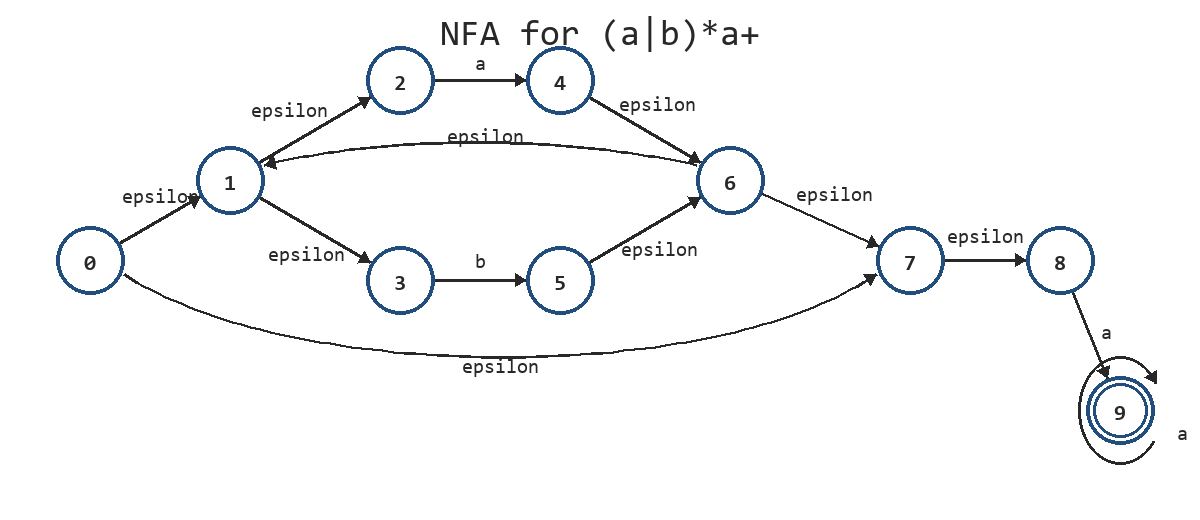
\includegraphics[width=0.82\linewidth]{figures/nfa-thompson-abstar-aplus.png}
\par{\small r = (a|b)*a+ 的 Thompson NFA}
\end{figure}

边表：

\begin{longtable}{|p{0.31\linewidth}|p{0.31\linewidth}|p{0.31\linewidth}|}
\hline
起点 & 边标号 & 终点 \\
\hline
\endfirsthead
起点 & 边标号 & 终点 \\
\hline
\endhead
0 & epsilon & 1 \\
\hline
0 & epsilon & 7 \\
\hline
1 & epsilon & 2 \\
\hline
1 & epsilon & 3 \\
\hline
2 & a & 4 \\
\hline
3 & b & 5 \\
\hline
4 & epsilon & 6 \\
\hline
5 & epsilon & 6 \\
\hline
6 & epsilon & 1 \\
\hline
6 & epsilon & 7 \\
\hline
7 & epsilon & 8 \\
\hline
8 & a & 9 \\
\hline
9 & a & 9 \\
\hline
\end{longtable}

起点是 \texttt{0}，终点是 \texttt{9}。

\paragraph*{3. 子集构造 DFA}

初态：

\begin{Verbatim}[fontsize=\small,breaklines=true]
A = epsilon-closure({0}) = {0,1,2,3,7,8}
\end{Verbatim}

从 A 出发：

\begin{Verbatim}[fontsize=\small,breaklines=true]
move(A,a) 包含 4 和 9，取 epsilon-closure 后得到 B
B = {1,2,3,4,6,7,8,9}

move(A,b) 包含 5，取 epsilon-closure 后得到 C
C = {1,2,3,5,6,7,8}
\end{Verbatim}

继续计算 B、C 的转移，得到：

\begin{longtable}{|p{0.19\linewidth}|p{0.19\linewidth}|p{0.19\linewidth}|p{0.19\linewidth}|p{0.19\linewidth}|}
\hline
DFA 状态 & NFA 状态集合 & on a & on b & 是否终态 \\
\hline
\endfirsthead
DFA 状态 & NFA 状态集合 & on a & on b & 是否终态 \\
\hline
\endhead
A & \texttt{\textbackslash{}\{0,1,2,3,7,8\textbackslash{}\}} & B & C & 否 \\
\hline
B & \texttt{\textbackslash{}\{1,2,3,4,6,7,8,9\textbackslash{}\}} & B & C & 是 \\
\hline
C & \texttt{\textbackslash{}\{1,2,3,5,6,7,8\textbackslash{}\}} & B & C & 否 \\
\hline
\end{longtable}

终态判断依据：集合中包含 NFA 终态 \texttt{9}。因此只有 B 是终态。

\begin{figure}[H]\centering
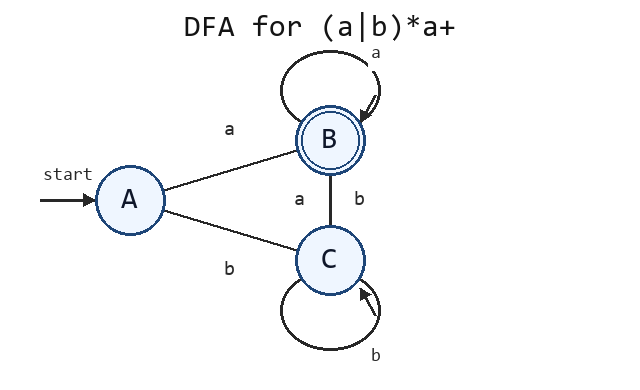
\includegraphics[width=0.82\linewidth]{figures/dfa-abstar-aplus.png}
\par{\small r = (a|b)*a+ 的 DFA}
\end{figure}

\paragraph*{4. 密码识别规则的正则表达式}

要求：

\begin{Verbatim}[fontsize=\small,breaklines=true]
字符只含 a,b,0,1
必须以字母开头
必须以 abb 结尾
中间不能出现连续两个数字
\end{Verbatim}

可写为：

\begin{Verbatim}[fontsize=\small,breaklines=true]
(a|b)((a|b)|0(a|b)|1(a|b))*abb
\end{Verbatim}

解释：

\begin{longtable}{|p{0.13\linewidth}|p{0.13\linewidth}|p{0.13\linewidth}|p{0.13\linewidth}|p{0.13\linewidth}|p{0.13\linewidth}|p{0.13\linewidth}|}
\hline
片段 & 作用 &  &  &  &  &  \\
\hline
\endfirsthead
片段 & 作用 &  &  &  &  &  \\
\hline
\endhead
`(a & b)` & 保证以字母开头 &  &  &  &  \\
\hline
`((a & b) & 0(a & b) & 1(a & b))*` & 中间部分中，数字后必须接字母，因此不会有连续两个数字 \\
\hline
\texttt{abb} & 保证以 \texttt{abb} 结尾 &  &  &  &  &  \\
\hline
\end{longtable}

该表达式中的每个字符都来自集合 \texttt{\textbackslash{}\{a,b,0,1\textbackslash{}\}}。

\subsection*{七、LL(1) 原题文法与二进制小数 SDD（20 分）}

\subsubsection*{题目}

给定文法：

\begin{Verbatim}[fontsize=\small,breaklines=true]
S -> c S | A B
A -> a A | epsilon
B -> b B a | d
\end{Verbatim}

1. 计算 FIRST 集和 FOLLOW 集。 2. 构造 LL(1) 预测分析表。 3. 判断该文法是否为 LL(1) 文法。

再给定文法：

\begin{Verbatim}[fontsize=\small,breaklines=true]
S -> L . L | L
L -> L B | B
B -> 0 | 1
\end{Verbatim}

4. 设计 SDD，计算二进制小数对应的十进制值。 5. 用该 SDD 计算 \texttt{101.101}。

\subsubsection*{按考试标准重写答案}

\paragraph*{1. FIRST 集}

文法：

\begin{Verbatim}[fontsize=\small,breaklines=true]
S -> c S | A B
A -> a A | epsilon
B -> b B a | d
\end{Verbatim}

先算 A、B：

\begin{longtable}{|p{0.23\linewidth}|p{0.23\linewidth}|p{0.23\linewidth}|p{0.23\linewidth}|}
\hline
非终结符 & 产生式 & FIRST &  \\
\hline
\endfirsthead
非终结符 & 产生式 & FIRST &  \\
\hline
\endhead
A & `A -> a A & epsilon` & \texttt{\textbackslash{}\{ a, epsilon \textbackslash{}\}} \\
\hline
B & `B -> b B a & d` & \texttt{\textbackslash{}\{ b, d \textbackslash{}\}} \\
\hline
\end{longtable}

再算 S：

\begin{Verbatim}[fontsize=\small,breaklines=true]
S -> c S          给出 c
S -> A B          A 可推出 epsilon，所以 FIRST(A B) = {a} union FIRST(B) = {a,b,d}
\end{Verbatim}

因此：

\begin{longtable}{|p{0.47\linewidth}|p{0.47\linewidth}|}
\hline
非终结符 & FIRST \\
\hline
\endfirsthead
非终结符 & FIRST \\
\hline
\endhead
S & \texttt{\textbackslash{}\{ a, b, c, d \textbackslash{}\}} \\
\hline
A & \texttt{\textbackslash{}\{ a, epsilon \textbackslash{}\}} \\
\hline
B & \texttt{\textbackslash{}\{ b, d \textbackslash{}\}} \\
\hline
\end{longtable}

\paragraph*{2. FOLLOW 集}

开始符号：

\begin{Verbatim}[fontsize=\small,breaklines=true]
FOLLOW(S) = { $ }
\end{Verbatim}

逐条产生式传播：

\begin{longtable}{|p{0.31\linewidth}|p{0.31\linewidth}|p{0.31\linewidth}|}
\hline
位置 & 推导依据 & 新增到 FOLLOW \\
\hline
\endfirsthead
位置 & 推导依据 & 新增到 FOLLOW \\
\hline
\endhead
\texttt{S -> A B} 中 A 后面是 B & 加入 FIRST(B) & \texttt{b,d} 加入 FOLLOW(A) \\
\hline
\texttt{S -> A B} 中 B 在末尾 & 加入 FOLLOW(S) & \texttt{\textbackslash{}\$} 加入 FOLLOW(B) \\
\hline
\texttt{B -> b B a} 中 B 后面是 a & 加入 \texttt{a} & \texttt{a} 加入 FOLLOW(B) \\
\hline
\end{longtable}

最终：

\begin{longtable}{|p{0.47\linewidth}|p{0.47\linewidth}|}
\hline
非终结符 & FOLLOW \\
\hline
\endfirsthead
非终结符 & FOLLOW \\
\hline
\endhead
S & \texttt{\textbackslash{}\{ \textbackslash{}\$ \textbackslash{}\}} \\
\hline
A & \texttt{\textbackslash{}\{ b, d \textbackslash{}\}} \\
\hline
B & \texttt{\textbackslash{}\{ a, \textbackslash{}\$ \textbackslash{}\}} \\
\hline
\end{longtable}

\paragraph*{3. 预测分析表}

填表依据：

\begin{longtable}{|p{0.31\linewidth}|p{0.31\linewidth}|p{0.31\linewidth}|}
\hline
产生式 & FIRST/FOLLOW 依据 & 填入表项 \\
\hline
\endfirsthead
产生式 & FIRST/FOLLOW 依据 & 填入表项 \\
\hline
\endhead
\texttt{S -> c S} & FIRST 为 \texttt{\textbackslash{}\{c\textbackslash{}\}} & \texttt{M[S,c]} \\
\hline
\texttt{S -> A B} & FIRST(A B) 为 \texttt{\textbackslash{}\{a,b,d\textbackslash{}\}} & \texttt{M[S,a]}，\texttt{M[S,b]}，\texttt{M[S,d]} \\
\hline
\texttt{A -> a A} & FIRST 为 \texttt{\textbackslash{}\{a\textbackslash{}\}} & \texttt{M[A,a]} \\
\hline
\texttt{A -> epsilon} & FOLLOW(A) 为 \texttt{\textbackslash{}\{b,d\textbackslash{}\}} & \texttt{M[A,b]}，\texttt{M[A,d]} \\
\hline
\texttt{B -> b B a} & FIRST 为 \texttt{\textbackslash{}\{b\textbackslash{}\}} & \texttt{M[B,b]} \\
\hline
\texttt{B -> d} & FIRST 为 \texttt{\textbackslash{}\{d\textbackslash{}\}} & \texttt{M[B,d]} \\
\hline
\end{longtable}

完整预测分析表，空白处为 error：

\begin{longtable}{|p{0.16\linewidth}|p{0.16\linewidth}|p{0.16\linewidth}|p{0.16\linewidth}|p{0.16\linewidth}|p{0.16\linewidth}|}
\hline
非终结符 & a & b & c & d & \$ \\
\hline
\endfirsthead
非终结符 & a & b & c & d & \$ \\
\hline
\endhead
S & \texttt{S -> A B} & \texttt{S -> A B} & \texttt{S -> c S} & \texttt{S -> A B} & error \\
\hline
A & \texttt{A -> a A} & \texttt{A -> epsilon} & error & \texttt{A -> epsilon} & error \\
\hline
B & error & \texttt{B -> b B a} & error & \texttt{B -> d} & error \\
\hline
\end{longtable}

\paragraph*{4. LL(1) 判断}

每个表项最多只有一条产生式，所以该文法是 LL(1) 文法。

\paragraph*{5. 二进制小数 SDD}

文法：

\begin{Verbatim}[fontsize=\small,breaklines=true]
S -> L . L | L
L -> L B | B
B -> 0 | 1
\end{Verbatim}

属性设计：

\begin{longtable}{|p{0.47\linewidth}|p{0.47\linewidth}|}
\hline
属性 & 含义 \\
\hline
\endfirsthead
属性 & 含义 \\
\hline
\endhead
\texttt{B.v} & 当前二进制位的值 \\
\hline
\texttt{L.v} & 当前二进制串按整数读法得到的值 \\
\hline
\texttt{L.len} & 当前二进制串长度 \\
\hline
\texttt{S.v} & 最终十进制值 \\
\hline
\end{longtable}

SDD：

\begin{Verbatim}[fontsize=\small,breaklines=true]
S -> L1 . L2
  S.v = L1.v + L2.v / 2 ^ L2.len

S -> L
  S.v = L.v

L -> L1 B
  L.v = 2 * L1.v + B.v
  L.len = L1.len + 1

L -> B
  L.v = B.v
  L.len = 1

B -> 0
  B.v = 0

B -> 1
  B.v = 1
\end{Verbatim}

\paragraph*{6. 计算 `101.101`}

左侧 \texttt{101}：

\begin{longtable}{|p{0.23\linewidth}|p{0.23\linewidth}|p{0.23\linewidth}|p{0.23\linewidth}|}
\hline
前缀 & 计算 & 值 & 长度 \\
\hline
\endfirsthead
前缀 & 计算 & 值 & 长度 \\
\hline
\endhead
\texttt{1} & \texttt{1} & 1 & 1 \\
\hline
\texttt{10} & \texttt{2*1+0} & 2 & 2 \\
\hline
\texttt{101} & \texttt{2*2+1} & 5 & 3 \\
\hline
\end{longtable}

右侧 \texttt{101} 同样按整数读法得到：

\begin{Verbatim}[fontsize=\small,breaklines=true]
L2.v = 5
L2.len = 3
\end{Verbatim}

代入：

\begin{Verbatim}[fontsize=\small,breaklines=true]
S.v = 5 + 5 / 2^3
    = 5 + 5/8
    = 5.625
\end{Verbatim}

最终十进制值是 \texttt{5.625}。

\subsection*{八、AST 构造 SDD 与语法树结点表示（20 分）}

\subsubsection*{题目}

给定表达式文法：

\begin{Verbatim}[fontsize=\small,breaklines=true]
E -> E + T | T
T -> T * F | F
F -> ( E ) | id
\end{Verbatim}

1. 设计构造 AST 的 SDD。 2. 说明 AST 结点对象通常需要保存哪些域。 3. 画出 \texttt{a + b * c} 的 AST。

\subsubsection*{按考试标准重写答案}

\paragraph*{1. 构造 AST 的 SDD}

原则：运算符产生式创建内部结点，括号不创建新结点，标识符创建叶子结点。

\begin{longtable}{|p{0.47\linewidth}|p{0.47\linewidth}|}
\hline
产生式 & 语义规则 \\
\hline
\endfirsthead
产生式 & 语义规则 \\
\hline
\endhead
\texttt{E -> E1 + T} & \texttt{E.node = Node("+", E1.node, T.node)} \\
\hline
\texttt{E -> T} & \texttt{E.node = T.node} \\
\hline
\texttt{T -> T1 * F} & \texttt{T.node = Node("*", T1.node, F.node)} \\
\hline
\texttt{T -> F} & \texttt{T.node = F.node} \\
\hline
\texttt{F -> ( E )} & \texttt{F.node = E.node} \\
\hline
\texttt{F -> id} & \texttt{F.node = Leaf(id.lexeme)} \\
\hline
\end{longtable}

该 SDD 是 S 属性定义，因为每个 \texttt{node} 都由子结点属性综合得到。

\paragraph*{2. AST 结点对象通常保存的域}

\begin{longtable}{|p{0.47\linewidth}|p{0.47\linewidth}|}
\hline
域 & 作用 \\
\hline
\endfirsthead
域 & 作用 \\
\hline
\endhead
\texttt{kind} 或 \texttt{op} & 表示结点类别，如 \texttt{+}、\texttt{*}、\texttt{id} \\
\hline
\texttt{children} & 指向子结点 \\
\hline
\texttt{name} 或 \texttt{value} & 叶子结点保存标识符名或常量值 \\
\hline
\texttt{type} & 类型检查后记录表达式类型 \\
\hline
\texttt{entry} & 标识符结点绑定符号表条目 \\
\hline
\texttt{sourceSpan} & 记录源码位置，便于报错 \\
\hline
\end{longtable}

\paragraph*{3. `a + b * c` 的 AST}

由于 \texttt{*} 优先级高于 \texttt{+}，所以 \texttt{b * c} 作为 \texttt{+} 的右子树：

\begin{figure}[H]\centering
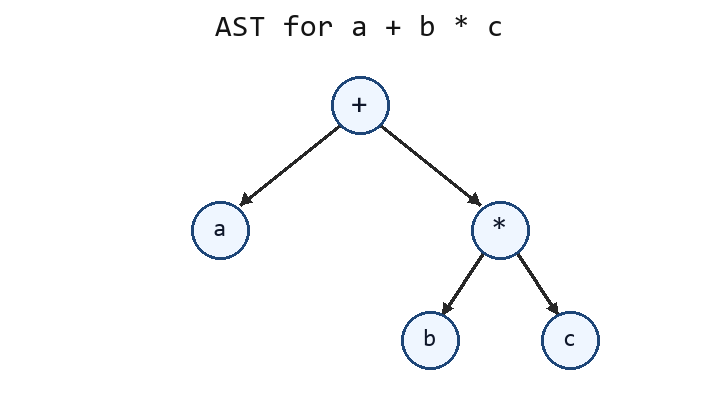
\includegraphics[width=0.82\linewidth]{figures/ast-a-plus-b-times-c.png}
\par{\small a + b * c 的 AST}
\end{figure}

\begin{Verbatim}[fontsize=\small,breaklines=true]
      +
     / \
    a   *
       / \
      b   c
\end{Verbatim}

构造过程：

\begin{longtable}{|p{0.47\linewidth}|p{0.47\linewidth}|}
\hline
子表达式 & AST 结点 \\
\hline
\endfirsthead
子表达式 & AST 结点 \\
\hline
\endhead
\texttt{a} & \texttt{Leaf(a)} \\
\hline
\texttt{b} & \texttt{Leaf(b)} \\
\hline
\texttt{c} & \texttt{Leaf(c)} \\
\hline
\texttt{b * c} & \texttt{Node("*", Leaf(b), Leaf(c))} \\
\hline
\texttt{a + b * c} & \texttt{Node("+", Leaf(a), Node("*", Leaf(b), Leaf(c)))} \\
\hline
\end{longtable}

\subsection*{九、IR 分类、设计维度与 phi 实现策略（20 分）}

\subsubsection*{题目}

回答下列问题：

1. 说明高层 IR、中层 IR、低层 IR 的区别。 2. 列出 IR 设计与分析的关键维度。 3. 说明树形 IR、三地址码、SSA、堆栈式 IR 的特点。 4. 说明 phi 函数在后端通常如何展开。

\subsubsection*{按考试标准重写答案}

\paragraph*{1. 高层 IR、中层 IR、低层 IR 的区别}

\begin{longtable}{|p{0.31\linewidth}|p{0.31\linewidth}|p{0.31\linewidth}|}
\hline
层次 & 特点 & 适合任务 \\
\hline
\endfirsthead
层次 & 特点 & 适合任务 \\
\hline
\endhead
高层 IR & 保留源语言结构，如函数、循环、对象、异常 & 语义分析、高层优化 \\
\hline
中层 IR & 抽象掉大部分源语言语法，常见为 TAC、四元式、SSA & 数据流分析、机器无关优化 \\
\hline
低层 IR & 接近机器，显式表示寄存器、栈、load/store、分支、调用约定 & 指令选择、寄存器分配、指令调度 \\
\hline
\end{longtable}

从高层到低层，源语言信息逐渐减少，机器细节逐渐增加。

\paragraph*{2. IR 设计与分析的关键维度}

\begin{longtable}{|p{0.47\linewidth}|p{0.47\linewidth}|}
\hline
维度 & 需要考虑的问题 \\
\hline
\endfirsthead
维度 & 需要考虑的问题 \\
\hline
\endhead
控制流表示 & 使用结构化控制流，还是基本块和显式跳转 \\
\hline
数据表示 & 使用临时变量、寄存器、栈操作数还是内存位置 \\
\hline
赋值模型 & 普通多次赋值，还是 SSA 静态单赋值 \\
\hline
类型信息 & 强类型 IR 还是弱类型 IR \\
\hline
内存模型 & 是否显式表示 load/store、指针、别名 \\
\hline
异常和运行时语义 & 是否保留异常、边界检查、GC 屏障 \\
\hline
可分析性 & 是否容易构造 CFG、DFG、def-use 链 \\
\hline
可生成性 & 是否容易映射到目标机器指令 \\
\hline
\end{longtable}

\paragraph*{3. 几种 IR 的特点}

\begin{longtable}{|p{0.23\linewidth}|p{0.23\linewidth}|p{0.23\linewidth}|p{0.23\linewidth}|}
\hline
IR 形式 & 特点 & 优点 & 局限 \\
\hline
\endfirsthead
IR 形式 & 特点 & 优点 & 局限 \\
\hline
\endhead
树形 IR & 用树表示表达式和语句结构 & 接近语法结构，适合前端 & 控制流和数据流不够显式 \\
\hline
三地址码 & 每条指令最多一个运算符 & 简单、线性、便于构造 CFG & 变量版本和 def-use 需要额外分析 \\
\hline
SSA & 每个变量版本只赋值一次，汇合处用 phi & 优化友好，def-use 清晰 & 后端前需要消除 phi \\
\hline
堆栈式 IR & 操作数隐含在栈上 & 指令紧凑 & 数据依赖不如三地址码显式 \\
\hline
\end{longtable}

\paragraph*{4. phi 函数在后端如何展开}

phi 的语义是在控制流汇合处按前驱边选择值：

\begin{Verbatim}[fontsize=\small,breaklines=true]
x3 = phi(x1 from L1, x2 from L2)
\end{Verbatim}

后端通常不能保留 phi，因此在前驱块末尾插入复制：

\begin{Verbatim}[fontsize=\small,breaklines=true]
L1:
  x1 = -1
  x3 = x1
  goto L3

L2:
  x2 = 1
  x3 = x2
  goto L3

L3:
  y = x3 * a
\end{Verbatim}

展开要点：

\begin{longtable}{|p{0.47\linewidth}|p{0.47\linewidth}|}
\hline
问题 & 处理方式 \\
\hline
\endfirsthead
问题 & 处理方式 \\
\hline
\endhead
phi 是并行赋值 & 多个 phi 同时展开时要避免复制顺序破坏值 \\
\hline
前驱边不能直接插入指令 & 拆分边，增加中间基本块 \\
\hline
复制可能冗余 & 寄存器分配时可合并不冲突的变量版本 \\
\hline
\end{longtable}

因此，phi 在 SSA 中用于表达数据流汇合，在后端变成普通 move 或被寄存器合并消除。

\subsection*{十、控制流翻译：穿越、回填表项与布尔值求值（20 分）}

\subsubsection*{题目}

回答并完成下列小题：

1. 说明 \texttt{truelist}、\texttt{falselist}、\texttt{nextlist} 的含义。 2. 说明 \texttt{makelist}、\texttt{merge}、\texttt{backpatch}、\texttt{nextquad} 的作用。 3. 说明标记非终结符 \texttt{M} 和 \texttt{N} 的作用。 4. 写出 \texttt{B1 \textbackslash{}\&\textbackslash{}\& B2}、\texttt{B1 || B2} 的回填规则。 5. 说明“穿越”和 \texttt{fall-through} 的关系。 6. 将赋值语句 \texttt{x = a < b \textbackslash{}\&\textbackslash{}\& c < d} 翻译为三地址码，要求得到布尔值 \texttt{0} 或 \texttt{1}。

\subsubsection*{按考试标准重写答案}

\paragraph*{1. `truelist`、`falselist`、`nextlist`}

\begin{longtable}{|p{0.31\linewidth}|p{0.31\linewidth}|p{0.31\linewidth}|}
\hline
列表 & 含义 & 常见来源 \\
\hline
\endfirsthead
列表 & 含义 & 常见来源 \\
\hline
\endhead
\texttt{B.truelist} & 布尔表达式 B 为真时应跳转、但目标未确定的指令位置 & \texttt{if relop goto \textbackslash{}\_} \\
\hline
\texttt{B.falselist} & 布尔表达式 B 为假时应跳转、但目标未确定的指令位置 & \texttt{goto \textbackslash{}\_} \\
\hline
\texttt{S.nextlist} & 语句 S 执行完后应跳到后继语句、但目标未确定的位置 & 语句末尾的跳转坯 \\
\hline
\end{longtable}

这些列表记录的是“待回填的指令编号”。

\paragraph*{2. `makelist`、`merge`、`backpatch`、`nextquad`}

\begin{longtable}{|p{0.47\linewidth}|p{0.47\linewidth}|}
\hline
函数或变量 & 作用 \\
\hline
\endfirsthead
函数或变量 & 作用 \\
\hline
\endhead
\texttt{makelist(i)} & 创建只含指令位置 \texttt{i} 的列表 \\
\hline
\texttt{merge(p1,p2)} & 合并两个待回填列表 \\
\hline
\texttt{backpatch(p,L)} & 把列表 \texttt{p} 中每条跳转指令的目标填成 \texttt{L} \\
\hline
\texttt{nextquad} & 下一条将要生成的三地址指令编号 \\
\hline
\end{longtable}

例子：

\begin{Verbatim}[fontsize=\small,breaklines=true]
100: if a < b goto _
101: goto _
\end{Verbatim}

此时：

\begin{Verbatim}[fontsize=\small,breaklines=true]
truelist = makelist(100)
falselist = makelist(101)
\end{Verbatim}

若真出口确定为 \texttt{120}，执行 \texttt{backpatch(truelist,120)} 后第 100 行目标变为 \texttt{120}。

\paragraph*{3. 标记非终结符 `M` 和 `N`}

\begin{Verbatim}[fontsize=\small,breaklines=true]
M -> epsilon
  M.instr = nextquad
\end{Verbatim}

\texttt{M} 不产生实际代码，用来记录“后面这段代码的起始位置”。

\begin{Verbatim}[fontsize=\small,breaklines=true]
N -> epsilon
  N.nextlist = makelist(nextquad)
  emit("goto _")
\end{Verbatim}

\texttt{N} 会生成一个尚未确定目标的 \texttt{goto}，用于跳过某段代码。

\begin{longtable}{|p{0.47\linewidth}|p{0.47\linewidth}|}
\hline
标记 & 作用 \\
\hline
\endfirsthead
标记 & 作用 \\
\hline
\endhead
M & 记录代码入口，供前面列表回填 \\
\hline
N & 生成跳转坯，避免 then 分支执行完后继续落入 else 分支 \\
\hline
\end{longtable}

\paragraph*{4. `B1 \&\& B2`、`B1 || B2` 的回填规则}

\texttt{\textbackslash{}\&\textbackslash{}\&}：只有 \texttt{B1} 为真时才检查 \texttt{B2}。

\begin{Verbatim}[fontsize=\small,breaklines=true]
B -> B1 && M B2
  backpatch(B1.truelist, M.instr)
  B.truelist = B2.truelist
  B.falselist = merge(B1.falselist, B2.falselist)
\end{Verbatim}

\texttt{||}：只有 \texttt{B1} 为假时才检查 \texttt{B2}。

\begin{Verbatim}[fontsize=\small,breaklines=true]
B -> B1 || M B2
  backpatch(B1.falselist, M.instr)
  B.truelist = merge(B1.truelist, B2.truelist)
  B.falselist = B2.falselist
\end{Verbatim}

关系运算的基本生成规则：

\begin{Verbatim}[fontsize=\small,breaklines=true]
B -> E1 relop E2
  B.truelist = makelist(nextquad)
  emit("if E1 relop E2 goto _")
  B.falselist = makelist(nextquad)
  emit("goto _")
\end{Verbatim}

\paragraph*{5. “穿越”和 fall-through 的关系}

穿越是语法制导翻译中的目标传递思想：把某个语句或布尔表达式的出口目标向下传给子结构。fall-through 是具体代码生成策略：不写显式 \texttt{goto}，让控制流自然进入下一条指令。

\begin{longtable}{|p{0.31\linewidth}|p{0.31\linewidth}|p{0.31\linewidth}|}
\hline
概念 & 层次 & 作用 \\
\hline
\endfirsthead
概念 & 层次 & 作用 \\
\hline
\endhead
穿越 & 翻译方案层面 & 传递目标标签 \\
\hline
fall-through & 生成代码层面 & 减少冗余跳转 \\
\hline
\end{longtable}

在控制流翻译中，可以把某个真出口或假出口设计为 fall-through，从而少生成一条 \texttt{goto}。

\paragraph*{6. `x = a < b \&\& c < d` 的布尔值求值}

这里右侧不是只控制分支，而是要得到布尔值 \texttt{0} 或 \texttt{1}，所以必须设置真分支赋 \texttt{1}，假分支赋 \texttt{0}。

短路逻辑：

\begin{longtable}{|p{0.31\linewidth}|p{0.31\linewidth}|p{0.31\linewidth}|}
\hline
子条件 & 为真时 & 为假时 \\
\hline
\endfirsthead
子条件 & 为真时 & 为假时 \\
\hline
\endhead
\texttt{a < b} & 继续判断 \texttt{c < d} & 整体为假 \\
\hline
\texttt{c < d} & 整体为真 & 整体为假 \\
\hline
\end{longtable}

三地址码：

\begin{Verbatim}[fontsize=\small,breaklines=true]
if a < b goto L_check2
goto L_false

L_check2:
if c < d goto L_true
goto L_false

L_true:
x = 1
goto L_next

L_false:
x = 0

L_next:
\end{Verbatim}

检查：

\begin{longtable}{|p{0.47\linewidth}|p{0.47\linewidth}|}
\hline
路径 & 结果 \\
\hline
\endfirsthead
路径 & 结果 \\
\hline
\endhead
\texttt{a < b} 为假 & 跳到 \texttt{L\textbackslash{}\_false}，\texttt{x=0} \\
\hline
\texttt{a < b} 为真且 \texttt{c < d} 为真 & 跳到 \texttt{L\textbackslash{}\_true}，\texttt{x=1} \\
\hline
\texttt{a < b} 为真且 \texttt{c < d} 为假 & 跳到 \texttt{L\textbackslash{}\_false}，\texttt{x=0} \\
\hline
\end{longtable}
\end{document}
